\documentclass[aspectratio=169,12pt,t]{beamer}

% --- Theme: Metropolis (modern, clean) ---
\usetheme[progressbar=frametitle,numbering=fraction,block=fill]{metropolis}

% --- Fira Sans font (install texlive-fonts-extra if missing) ---
\IfFileExists{FiraSans.sty}{\usepackage[sfdefault]{FiraSans}}{}

% --- Light background with warm accent ---
\definecolor{mDarkTeal}{RGB}{35,55,59}
\definecolor{mLightBrown}{RGB}{235,228,216}
\definecolor{mAccent}{RGB}{140,70,20}

\setbeamercolor{normal text}{fg=mDarkTeal,bg=white}
\setbeamercolor{alerted text}{fg=mAccent}
\setbeamercolor{frametitle}{bg=mDarkTeal,fg=white}
\setbeamercolor{progress bar}{fg=mAccent,bg=mLightBrown}
\setbeamercolor{title separator}{fg=mAccent}
\setbeamercolor{progress bar in head/foot}{fg=mAccent,bg=mLightBrown}
\setbeamercolor{progress bar in section page}{fg=mAccent,bg=mLightBrown}

% --- Packages ---
\usepackage[utf8]{inputenc}
\usepackage{amsmath,amssymb,amsthm}
\usepackage{mathrsfs}
\usepackage{tikz}
\usetikzlibrary{arrows.meta,positioning,calc,decorations.pathreplacing,shapes,patterns}
\usepackage{pgfplots}
\pgfplotsset{compat=1.18}

% --- Custom colors for content types ---
\definecolor{defcolor}{RGB}{25,85,120}
\definecolor{thmcolor}{RGB}{140,35,35}
\definecolor{proofcolor}{RGB}{35,100,50}
\definecolor{excolor}{RGB}{140,75,10}
\definecolor{remcolor}{RGB}{90,90,90}

% --- Beamer blocks for mathematical content types ---
\newenvironment{defblock}[1]{%
  \setbeamercolor{block title}{bg=defcolor,fg=white}%
  \setbeamercolor{block body}{bg=defcolor!5}%
  \begin{block}{#1}}{\end{block}}

\newenvironment{thmblock}[1]{%
  \setbeamercolor{block title}{bg=thmcolor,fg=white}%
  \setbeamercolor{block body}{bg=thmcolor!5}%
  \begin{block}{#1}}{\end{block}}

\newenvironment{proofblock}[1]{%
  \setbeamercolor{block title}{bg=proofcolor,fg=white}%
  \setbeamercolor{block body}{bg=proofcolor!5}%
  \begin{block}{#1}}{\end{block}}

\newenvironment{exblock}[1]{%
  \setbeamercolor{block title}{bg=excolor,fg=white}%
  \setbeamercolor{block body}{bg=excolor!5}%
  \begin{block}{#1}}{\end{block}}

\newenvironment{remblock}[1]{%
  \setbeamercolor{block title}{bg=remcolor,fg=white}%
  \setbeamercolor{block body}{bg=remcolor!5}%
  \begin{block}{#1}}{\end{block}}

% --- Metadata ---
\title{Chapter 2: Basic Topology}
\subtitle{Section: Perfect Sets}
\author{Based on Walter Rudin's \emph{Principles of Mathematical Analysis}}
\date{}

\begin{document}

% =============================================================================
\begin{frame}
  \titlepage
  \note{
    Welcome back to Chapter 2 of Principles of Mathematical Analysis. In this
    section we study perfect sets. A perfect set is a closed set in which every
    point is a limit point, so there are no isolated points. These look like
    small, rigid objects, but we will see that they are always very large in a
    specific sense: every nonempty perfect set in Euclidean space is
    uncountable. As a striking application we will build the Cantor set, a
    perfect subset of the unit interval that contains no segment at all, yet
    is still uncountable. It is one of the most famous examples in analysis
    and in topology.
  }
\end{frame}

% =============================================================================
\begin{frame}{Outline}
  \tableofcontents
  \note{
    Here is the plan. We start with a short motivation for why perfect sets
    deserve a dedicated section. Then we state and prove Theorem 2.43, which
    says that every nonempty perfect set in "R" to the "k" is uncountable. As
    an immediate corollary we get that every closed interval with more than
    one point, and therefore the entire real line, is uncountable. The second
    half of the section is devoted to the Cantor set: its construction, its
    properties, and why it is perfect even though it contains no segment at
    all.
  }
\end{frame}

% =============================================================================
% --- Motivation ---
% =============================================================================

% --- Build 1/3 ---
\begin{frame}{Why Perfect Sets Matter}
  \begin{itemize}
    \item A \alert{perfect} set is closed with \emph{no isolated points}
  \end{itemize}
  \note{
    Recall from Definition 2.18 that a set is perfect if it is closed and
    every point of the set is also a limit point. In plain terms, every
    point has other points of the set arbitrarily close by. There are no
    lonely points floating off on their own. This definition sounds mild,
    but it is the only hypothesis we need to conclude something very strong.
  }
\end{frame}

% --- Build 2/3 ---
\begin{frame}{Why Perfect Sets Matter}
  \begin{itemize}
    \item A \alert{perfect} set is closed with \emph{no isolated points}
    \item Every nonempty perfect set in $\mathbb{R}^k$ is \alert{uncountable}
  \end{itemize}
  \note{
    The main result of this section is that every nonempty perfect subset of
    Euclidean space is uncountable. So once a closed set packs itself
    together densely enough that every point has neighbors, it must already
    contain continuum many points. This is a beautiful bridge between the
    topological property of no isolated points and the set theoretic
    property of uncountability.
  }
\end{frame}

% --- Build 3/3 ---
\begin{frame}{Why Perfect Sets Matter}
  \begin{itemize}
    \item A \alert{perfect} set is closed with \emph{no isolated points}
    \item Every nonempty perfect set in $\mathbb{R}^k$ is \alert{uncountable}
    \item The \alert{Cantor set}: perfect, uncountable, contains no interval
  \end{itemize}
  \note{
    Then we turn to the headline example: the Cantor set. It lives inside
    the unit interval, it contains no segment whatsoever, and yet it is
    perfect. By our theorem it must therefore be uncountable. The Cantor set
    is the prototype for many pathological examples later in the book, and
    in measure theory it gives an uncountable set of measure zero. Let us
    now make everything precise.
  }
\end{frame}

% =============================================================================
\section{The Main Theorem}
% =============================================================================

% =============================================================================
% --- Recall: Perfect Set Definition ---
% =============================================================================

\begin{frame}{Recall: Definition 2.18(h) --- Perfect Set}
  \begin{defblock}{Definition (Perfect Set)}
    A set $E$ in a metric space $X$ is \alert{perfect} if
    \begin{enumerate}
      \item[(1)] $E$ is closed, and
      \item[(2)] every point of $E$ is a \emph{limit point} of $E$.
    \end{enumerate}
  \end{defblock}

  \vspace{0.5em}
  \textbf{Equivalent form:} $E$ is perfect $\iff$ $E$ has no isolated points and contains all its limit points.

  \note{
    Before we prove anything, let us remind ourselves what a perfect set is.
    The slide lists the two conditions. First, "E" must be closed, meaning
    it contains all of its limit points. Second, every point of "E" must be
    a limit point of "E", meaning every neighborhood of any point of "E"
    contains other points of "E". Combining the two, "E" has no isolated
    points and contains all its limit points. The two famous examples to
    keep in mind are any closed interval with positive length, and all of
    "R" to the "k". In the exercises we will see more exotic examples.
  }
\end{frame}

% =============================================================================
% --- Theorem 2.43 Statement ---
% =============================================================================

\begin{frame}{Theorem 2.43: Perfect Sets Are Uncountable}
  \begin{thmblock}{Theorem 2.43}
    Let $P$ be a nonempty \alert{perfect} set in $\mathbb{R}^k$.\\
    Then $P$ is \alert{uncountable}.
  \end{thmblock}

  \vspace{0.8em}
  \textbf{Contrast:} A countable set can still be closed --- e.g.\ $\mathbb{Z}$ or $\{1/n\} \cup \{0\}$.

  \vspace{0.4em}
  What fails for these sets? They have \emph{isolated points}.

  \note{
    Here is the theorem. Take any nonempty perfect set "P" sitting inside "R"
    to the "k". The conclusion is that "P" is uncountable, meaning its
    cardinality is at least that of the real line. Notice how little we are
    assuming about "P". We do not require it to be bounded, we do not
    require it to contain any segment, and we do not require it to be convex
    or nicely shaped. The only input is that it is closed with no isolated
    points. Compare this with the integers, which are closed but entirely
    made of isolated points, or with the set of zero together with 1 over
    "n", which has a limit point at zero but is still countable. Perfection
    is exactly the condition that rules out such countable closed sets.
  }
\end{frame}

% =============================================================================
% --- Proof Strategy ---
% =============================================================================

\begin{frame}{Proof Strategy: Theorem 2.43}
  \textbf{Approach:} \alert{Proof by contradiction}, using compactness.

  \vspace{0.8em}
  \textbf{Setup:} Assume $P$ is countable, so
  \[
    P = \{\mathbf{x}_1, \mathbf{x}_2, \mathbf{x}_3, \dots\}.
  \]

  \vspace{0.4em}
  \textbf{Plan:} Build a shrinking sequence of neighborhoods $V_1 \supset V_2 \supset \cdots$ such that
  \begin{itemize}
    \item each $V_n$ meets $P$,
    \item $\overline{V}_{n+1}$ \alert{excludes} $\mathbf{x}_n$ --- so no listed point lies in every $\overline{V}_n$.
  \end{itemize}
  Then nested \emph{compact} sets $K_n = \overline{V}_n \cap P$ must share a point of $P$ --- \alert{contradiction}.

  \note{
    The proof is a contradiction argument with a compactness twist. We
    suppose for contradiction that "P" is countable, so we can list all its
    points as "x" sub 1, "x" sub 2, "x" sub 3, and so on. The idea is to
    construct an infinite sequence of open balls, each with its closure
    sitting strictly inside the previous ball, and to do this so that two
    features hold. First, each ball meets "P", so the closures intersected
    with "P" are all nonempty compact sets. Second, by the time we reach
    the "n" plus first ball, we have excluded the "n"-th listed point of
    "P" from its closure, so no listed point survives in all of the nested
    compact sets. The corollary to Theorem 2.36 says nested nonempty
    compact sets have nonempty intersection. That intersection lies in
    "P", so it must contain some listed point; but we just kicked every
    listed point out. That is our contradiction. Let us work through each
    piece.
  }
\end{frame}

% =============================================================================
% --- Proof: Base Case V_1 ---
% =============================================================================

\begin{frame}{Proof --- Step 1: The Base Case}
  \begin{proofblock}{Step 1: Choose $V_1$}
    Let $V_1$ be \emph{any} neighborhood of $\mathbf{x}_1$:
    \[
      V_1 = \{\mathbf{y} \in \mathbb{R}^k : |\mathbf{y} - \mathbf{x}_1| < r\}.
    \]
    Its closure is the closed ball
    \[
      \overline{V}_1 = \{\mathbf{y} \in \mathbb{R}^k : |\mathbf{y} - \mathbf{x}_1| \leq r\}.
    \]
  \end{proofblock}

  \vspace{0.4em}
  Since $\mathbf{x}_1 \in P$, we have $V_1 \cap P \neq \emptyset$.

  \note{
    We start by choosing any open ball around the first listed point "x" sub
    1, and we call that ball "V" sub 1. The radius can be anything positive,
    it does not matter for the construction. The closure of "V" sub 1 is the
    corresponding closed ball with the boundary attached, shown on the
    slide. The key observation is that "x" sub 1 itself belongs to "P", so
    the open ball "V" sub 1 meets "P". This is the induction hypothesis we
    will propagate.
  }
\end{frame}

% =============================================================================
% --- Proof: Inductive Step (build 1/4) ---
% =============================================================================

% --- Build 1/4 ---
\begin{frame}{Proof --- Step 2: The Inductive Step}
  \begin{proofblock}{Step 2: Build $V_{n+1}$ from $V_n$}
    \textbf{Inductive hypothesis:} $V_n$ is a neighborhood with $V_n \cap P \neq \emptyset$.
  \end{proofblock}

  \vspace{0.6em}
  We want to construct $V_{n+1}$ satisfying:
  \begin{enumerate}
    \item[(i)] $\overline{V}_{n+1} \subset V_n$
  \end{enumerate}

  \note{
    Now for the inductive step. Suppose we have already constructed "V"
    sub "n" and it meets "P". Our goal is to choose a smaller neighborhood
    "V" sub "n" plus 1 with three properties. The first property is that
    the closure of "V" sub "n" plus 1 sits strictly inside "V" sub "n".
    This makes the sequence of closures a genuinely nested decreasing
    sequence, which is what we need for the compactness argument at the
    end.
  }
\end{frame}

% --- Build 2/4 ---
\begin{frame}{Proof --- Step 2: The Inductive Step}
  \begin{proofblock}{Step 2: Build $V_{n+1}$ from $V_n$}
    \textbf{Inductive hypothesis:} $V_n$ is a neighborhood with $V_n \cap P \neq \emptyset$.
  \end{proofblock}

  \vspace{0.6em}
  We want to construct $V_{n+1}$ satisfying:
  \begin{enumerate}
    \item[(i)] $\overline{V}_{n+1} \subset V_n$
    \item[(ii)] $\mathbf{x}_n \notin \overline{V}_{n+1}$ \quad \alert{(kick out the $n$-th listed point)}
  \end{enumerate}

  \note{
    The second property is the clever part. We insist that "x" sub
    "n", the "n"-th listed point of "P", is not in the closure of "V" sub
    "n" plus 1. In other words, we kick the "n"-th point of "P" out of our
    closed ball. Over the course of the induction, we will have kicked out
    every listed point of "P", so nothing in our countable listing can
    survive in every closure.
  }
\end{frame}

% --- Build 3/4 ---
\begin{frame}{Proof --- Step 2: The Inductive Step}
  \begin{proofblock}{Step 2: Build $V_{n+1}$ from $V_n$}
    \textbf{Inductive hypothesis:} $V_n$ is a neighborhood with $V_n \cap P \neq \emptyset$.
  \end{proofblock}

  \vspace{0.6em}
  We want to construct $V_{n+1}$ satisfying:
  \begin{enumerate}
    \item[(i)] $\overline{V}_{n+1} \subset V_n$
    \item[(ii)] $\mathbf{x}_n \notin \overline{V}_{n+1}$ \quad \alert{(kick out the $n$-th listed point)}
    \item[(iii)] $V_{n+1} \cap P \neq \emptyset$ \quad \alert{(propagate the hypothesis)}
  \end{enumerate}

  \note{
    The third property is what we need to run the induction again:
    the new neighborhood must also meet "P". Without this we could not
    continue the construction past step "n" plus 1. Now, can we really
    always achieve all three simultaneously? That is where perfection of
    "P" enters the argument.
  }
\end{frame}

% --- Build 4/4 ---
\begin{frame}{Proof --- Step 2: The Inductive Step}
  \begin{proofblock}{Why this is possible}
    Pick any $\mathbf{p} \in V_n \cap P$. Since $P$ is \alert{perfect}, $\mathbf{p}$ is a limit point of $P$, so arbitrarily small neighborhoods of $\mathbf{p}$ contain many points of $P$.
  \end{proofblock}

  \vspace{0.5em}
  Choose $\mathbf{q} \in P$ with $\mathbf{q} \neq \mathbf{x}_n$ arbitrarily close to $\mathbf{p}$.\\
  Take $V_{n+1}$ a tiny ball around $\mathbf{q}$ whose closure:
  \begin{itemize}
    \item stays inside $V_n$ \hfill [gives (i)]
    \item misses $\mathbf{x}_n$ \hfill [gives (ii)]
  \end{itemize}
  Since $\mathbf{q} \in V_{n+1} \cap P$, we have (iii).

  \note{
    Here is the construction, powered by perfection. Take any point "p" of
    "P" inside "V" sub "n", which exists by the inductive hypothesis. Since
    "P" is perfect, "p" is a limit point of "P", so every neighborhood of
    "p" contains infinitely many points of "P" by Theorem 2.20. Pick a
    point "q" of "P" near "p" but different from "x" sub "n". Then take a
    small open ball around "q" whose closure stays inside "V" sub "n" and
    does not touch "x" sub "n". Call that ball "V" sub "n" plus 1.
    The first two conditions are built in by the choice of radius, and
    the third condition holds because "q" itself is in "V" sub "n" plus 1
    and in "P". The induction proceeds.
  }
\end{frame}

% =============================================================================
% --- Proof: Diagram of Shrinking Neighborhoods ---
% =============================================================================

\begin{frame}{Visualizing the Shrinking Neighborhoods}
  \begin{center}
  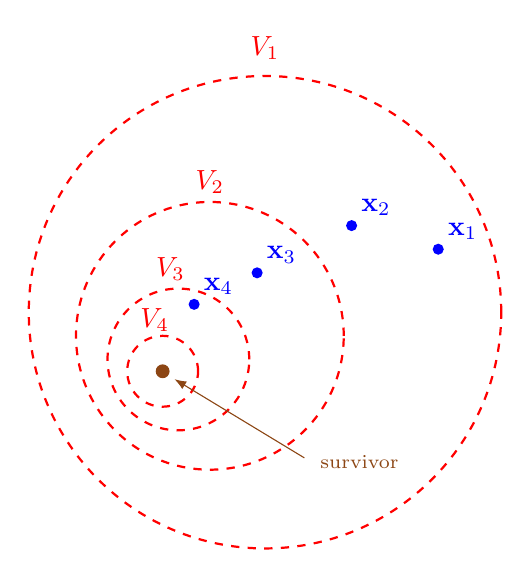
\begin{tikzpicture}[scale=1.0]
    % Outer ball V_1
    \draw[thick, red, dashed] (0,0) circle (3);
    \node[red] at (0, 3.35) {$V_1$};

    % V_2 inside V_1
    \draw[thick, red, dashed] (-0.7,-0.3) circle (1.7);
    \node[red] at (-0.7, 1.65) {$V_2$};

    % V_3 inside V_2
    \draw[thick, red, dashed] (-1.1,-0.6) circle (0.9);
    \node[red] at (-1.2, 0.55) {$V_3$};

    % V_4 inside V_3
    \draw[thick, red, dashed] (-1.3,-0.75) circle (0.45);
    \node[red] at (-1.4, -0.1) {$V_4$};

    % Points x_1, x_2, x_3 -- each excluded by next shell
    \fill[blue] (2.2,0.8) circle (2pt) node[above right]{$\mathbf{x}_1$};
    \fill[blue] (1.1,1.1) circle (2pt) node[above right]{$\mathbf{x}_2$};
    \fill[blue] (-0.1,0.5) circle (2pt) node[above right]{$\mathbf{x}_3$};
    \fill[blue] (-0.9,0.1) circle (2pt) node[above right]{$\mathbf{x}_4$};

    % A point of P that survives
    \fill[mAccent] (-1.3,-0.75) circle (2.5pt);
    \node[mAccent, font=\scriptsize] at (1.2,-1.9) {survivor};
    \draw[mAccent, thin, -{Latex[length=1.5mm]}] (0.5,-1.85) -- (-1.15,-0.85);
  \end{tikzpicture}
  \end{center}

  \note{
    This picture shows the idea behind the construction. The four red
    dashed circles are successive open balls "V" sub 1, "V" sub 2, "V" sub
    3, "V" sub 4, each with its closure strictly inside the previous one.
    The blue dots are the listed points of "P", namely "x" sub 1, "x" sub
    2, "x" sub 3, "x" sub 4. Notice that "x" sub 1 sits inside "V" sub 1
    but is kicked out once we pass to "V" sub 2. At each successive step
    we steer the next ball so that its closure excludes the next listed
    point. So after a few steps, none of "x" sub 1, "x" sub 2, "x" sub 3,
    or "x" sub 4 remain in the inner balls. The orange dot in the center
    represents the target of the nesting, a point that should survive all
    intersections. Compactness will tell us that such a surviving point
    actually exists.
  }
\end{frame}

% =============================================================================
% --- Proof: Step 3 Define K_n ---
% =============================================================================

\begin{frame}{Proof --- Step 3: Compact Pieces $K_n$}
  \begin{proofblock}{Define}
    \[
      K_n = \overline{V}_n \cap P
    \]
  \end{proofblock}

  \vspace{0.4em}
  \textbf{Each $K_n$ is compact:}
  \begin{itemize}
    \item $\overline{V}_n$ is \alert{closed and bounded} in $\mathbb{R}^k$ $\Longrightarrow$ compact (Heine--Borel).
    \item $P$ is closed.
    \item $K_n = \overline{V}_n \cap P$ is a closed subset of a compact set $\Longrightarrow$ compact (Thm 2.35).
  \end{itemize}

  \note{
    Now we switch from open neighborhoods to compact building blocks. Define
    "K" sub "n" to be the closure of "V" sub "n" intersected with "P". Each
    "K" sub "n" is compact, for two reasons on the slide. First, the closure
    of "V" sub "n" is a closed ball, hence closed and bounded in Euclidean
    space, which makes it compact by the Heine-Borel theorem. Second, "P"
    is closed by perfection, so the intersection of a closed set and a
    compact set is a closed subset of a compact set, which is again compact
    by Theorem 2.35. So each "K" sub "n" is a compact subset of "P".
  }
\end{frame}

% =============================================================================
% --- Proof: Nested and Nonempty (build 1/3) ---
% =============================================================================

% --- Build 1/3 ---
\begin{frame}{Proof --- Step 4: Reaching a Contradiction}
  \begin{proofblock}{Properties of $\{K_n\}$}
    \begin{itemize}
      \item[(a)] Each $K_n$ is \alert{nonempty}: by (iii), $V_n \cap P \neq \emptyset$, so $K_n \supset V_n \cap P \neq \emptyset$.
    \end{itemize}
  \end{proofblock}

  \note{
    We will show that the compact sets "K" sub "n" satisfy the hypotheses of
    the corollary to Theorem 2.36, but their intersection is nevertheless
    empty. That corollary says nested nonempty compact sets cannot have
    empty intersection, so we will have a contradiction. First, each "K" sub
    "n" is nonempty. This is because "V" sub "n" meets "P" by the third
    condition of our construction, and "K" sub "n" is even larger than
    "V" sub "n" intersected with "P", since it uses the closure. So "K"
    sub "n" is nonempty.
  }
\end{frame}

% --- Build 2/3 ---
\begin{frame}{Proof --- Step 4: Reaching a Contradiction}
  \begin{proofblock}{Properties of $\{K_n\}$}
    \begin{itemize}
      \item[(a)] Each $K_n$ is \alert{nonempty}: by (iii), $V_n \cap P \neq \emptyset$, so $K_n \supset V_n \cap P \neq \emptyset$.
      \item[(b)] $K_n \supset K_{n+1}$: by (i), $\overline{V}_{n+1} \subset V_n \subset \overline{V}_n$.
    \end{itemize}
  \end{proofblock}

  \note{
    Second, the sets are nested. By the first condition of our
    construction, the closure of "V" sub "n" plus 1 lies in "V" sub "n",
    hence in the closure of "V" sub "n". So intersecting with "P" gives
    "K" sub "n" plus 1 as a subset of "K" sub "n". The sequence "K" sub
    1, "K" sub 2, "K" sub 3, and so on, is a decreasing chain of nonempty
    compact sets.
  }
\end{frame}

% --- Build 3/3 ---
\begin{frame}{Proof --- Step 4: Reaching a Contradiction}
  \begin{proofblock}{Properties of $\{K_n\}$}
    \begin{itemize}
      \item[(a)] Each $K_n$ is \alert{nonempty}
      \item[(b)] $K_n \supset K_{n+1}$
      \item[(c)] $\mathbf{x}_n \notin K_{n+1}$: by (ii), $\mathbf{x}_n \notin \overline{V}_{n+1}$, so $\mathbf{x}_n \notin K_{n+1}$.
    \end{itemize}
  \end{proofblock}

  \vspace{0.3em}
  Therefore \alert{no listed point} $\mathbf{x}_n$ lies in $\bigcap_{m=1}^{\infty} K_m$, so
  \[
    \bigcap_{m=1}^{\infty} K_m \;\cap\; P \;=\; \emptyset.
  \]
  But $K_m \subset P$ for all $m$, so $\bigcap_{m=1}^{\infty} K_m = \emptyset$.

  \note{
    Third, and this is the key observation, for each "n" the point "x" sub
    "n" is not in "K" sub "n" plus 1. This is exactly the second
    condition of our construction, phrased in terms of "K". So "x" sub
    "n" is missing from "K" sub "n" plus
    1 and therefore, by nesting, from every "K" sub "m" with "m" bigger
    than "n". So "x" sub "n" is not in the total intersection. Since every
    point of "P" appears somewhere in our list, no point of "P" is in the
    intersection. But the "K" sub "m" are all subsets of "P", so their
    intersection is a subset of "P" that contains no point of "P". In other
    words, the intersection is empty.
  }
\end{frame}

% =============================================================================
% --- Proof: The Contradiction ---
% =============================================================================

\begin{frame}{Proof --- Conclusion}
  We have a sequence of \alert{nonempty} nested \alert{compact} sets
  \[
    K_1 \supset K_2 \supset K_3 \supset \cdots
  \]
  with $\displaystyle \bigcap_{n=1}^{\infty} K_n = \emptyset$.

  \vspace{0.6em}
  \textbf{But} the \emph{Corollary to Theorem 2.36} says
  \[
    \bigcap_{n=1}^{\infty} K_n \neq \emptyset.
  \]

  \vspace{0.4em}
  \centerline{\alert{Contradiction!} $\qquad\boxed{P \text{ cannot be countable.}}$}

  \note{
    We have reached a contradiction. The corollary to Theorem 2.36 stated
    that a nested decreasing sequence of nonempty compact sets has nonempty
    intersection. Our "K" sub "n" are nonempty, nested, and compact, so
    their intersection should be nonempty. But we just showed it is empty.
    The only way to avoid this contradiction is to reject the assumption
    that "P" is countable. Therefore every nonempty perfect set in "R" to
    the "k" is uncountable. The theorem is proved.
  }
\end{frame}

% =============================================================================
% --- Corollary ---
% =============================================================================

\begin{frame}{Corollary: $\mathbb{R}$ is Uncountable}
  \begin{thmblock}{Corollary}
    Every interval $[a,b]$ with $a<b$ is \alert{uncountable}.\\
    In particular, $\mathbb{R}$ is uncountable.
  \end{thmblock}

  \vspace{0.8em}
  \textbf{Why:} $[a,b] \subset \mathbb{R}$ is
  \begin{itemize}
    \item closed,
    \item every point is a limit point (interior points approached from both sides; endpoints from inside),
  \end{itemize}
  so $[a,b]$ is \alert{perfect}. Apply Theorem 2.43.

  \note{
    As an immediate consequence we get a classical result: every closed
    interval with distinct endpoints is uncountable, and therefore the
    real line itself is uncountable. The reason is that such an interval
    is perfect. It is closed, and every one of its points is a limit
    point. An interior point has other points of the interval on both
    sides approaching it, while each endpoint has points of the interval
    approaching it from inside. Since there are no isolated points,
    Theorem 2.43 applies and tells us the interval is uncountable. This
    gives a second proof of the uncountability of the real numbers, using
    topology rather than a diagonal argument.
  }
\end{frame}

% =============================================================================
\section{The Cantor Set}
% =============================================================================

% =============================================================================
% --- Cantor Set Motivation ---
% =============================================================================

\begin{frame}{2.44 --- The Cantor Set}
  \textbf{Goal:} Exhibit a perfect set in $\mathbb{R}^1$ that contains \alert{no segment}.

  \vspace{0.8em}
  \textbf{Why is this surprising?}

  \vspace{0.3em}
  \begin{itemize}
    \item The obvious perfect subsets of $\mathbb{R}$ --- closed intervals --- are ``thick''.
    \item Can we have a perfect set that is so ``thin'' it contains no interval?
  \end{itemize}

  \vspace{0.5em}
  \textbf{Answer:} Yes --- the \alert{Cantor set}.

  \note{
    To round out the section, Rudin constructs the most famous example of
    a perfect set, the Cantor set. The surprise is this: the obvious
    perfect subsets of the real line, like a closed interval, are what we
    might call thick, because they contain open intervals. Is there a
    perfect set so thin that it contains no interval at all? The answer
    is yes, and the Cantor construction will build one. Once we have it,
    our main theorem automatically tells us it is uncountable, giving a
    strange little set that is as small as possible in one sense and as
    big as possible in another.
  }
\end{frame}

% =============================================================================
% --- Construction (progressive build) ---
% =============================================================================

% --- Build 1/4 ---
\begin{frame}{Construction: Removing Middle Thirds}
  \textbf{Start with:}
  \[
    E_0 = [0,1].
  \]

  \vspace{0.5em}
  \begin{center}
  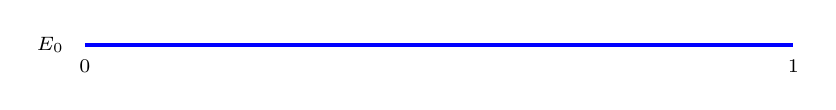
\begin{tikzpicture}[scale=9]
    \draw[very thick, blue] (0,0) -- (1,0);
    \node[below=2pt] at (0,0) {\scriptsize $0$};
    \node[below=2pt] at (1,0) {\scriptsize $1$};
    \node[left=4pt] at (0,0) {\scriptsize $E_0$};
  \end{tikzpicture}
  \end{center}

  \note{
    The construction proceeds in stages. Stage zero is easy: "E" sub zero
    is just the closed unit interval from 0 to 1, shown as the blue bar on
    the slide. At each subsequent stage we will delete the open middle
    third of every interval present, leaving a shorter, more fragmented
    set. Let us watch the first few stages.
  }
\end{frame}

% --- Build 2/4 ---
\begin{frame}{Construction: Removing Middle Thirds}
  \textbf{Stage 1:} remove the open segment $(\tfrac{1}{3},\tfrac{2}{3})$.
  \[
    E_1 = [0,\tfrac{1}{3}] \cup [\tfrac{2}{3},1].
  \]

  \vspace{0.5em}
  \begin{center}
  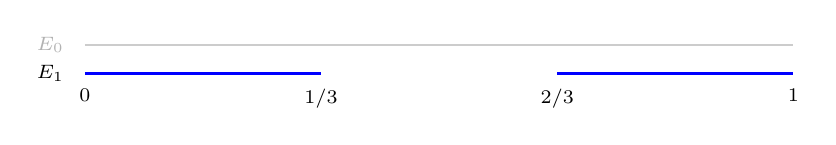
\begin{tikzpicture}[scale=9]
    % E_0 faint
    \draw[thick, gray!40] (0,0.04) -- (1,0.04);
    \node[gray!60, left=4pt] at (0,0.04) {\scriptsize $E_0$};
    % E_1
    \draw[very thick, blue] (0,0) -- (1/3,0);
    \draw[very thick, blue] (2/3,0) -- (1,0);
    \node[below=2pt] at (0,0) {\scriptsize $0$};
    \node[below=2pt] at (1/3,0) {\scriptsize $1/3$};
    \node[below=2pt] at (2/3,0) {\scriptsize $2/3$};
    \node[below=2pt] at (1,0) {\scriptsize $1$};
    \node[left=4pt] at (0,0) {\scriptsize $E_1$};
  \end{tikzpicture}
  \end{center}

  \note{
    At stage 1 we remove the open middle third of the unit interval, that
    is, the open segment from 1 over 3 to 2 over 3. What remains is "E"
    sub 1, the union of two closed intervals, the left third and the right
    third. On the picture, the grey bar above is "E" sub zero for
    reference, and the blue pieces below are "E" sub 1.
  }
\end{frame}

% --- Build 3/4 ---
\begin{frame}{Construction: Removing Middle Thirds}
  \textbf{Stage 2:} remove the middle thirds of each remaining interval.
  \[
    E_2 = [0,\tfrac{1}{9}] \cup [\tfrac{2}{9},\tfrac{3}{9}] \cup [\tfrac{6}{9},\tfrac{7}{9}] \cup [\tfrac{8}{9},1].
  \]

  \vspace{0.5em}
  \begin{center}
  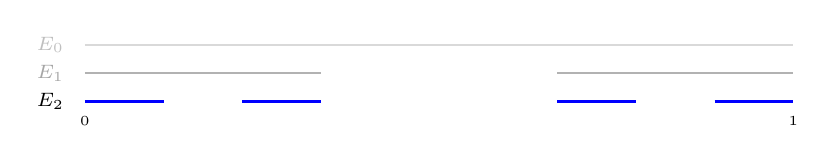
\begin{tikzpicture}[scale=9]
    % E_0
    \draw[thick, gray!30] (0,0.08) -- (1,0.08);
    \node[gray!50, left=4pt] at (0,0.08) {\scriptsize $E_0$};
    % E_1
    \draw[thick, gray!60] (0,0.04) -- (1/3,0.04);
    \draw[thick, gray!60] (2/3,0.04) -- (1,0.04);
    \node[gray!70, left=4pt] at (0,0.04) {\scriptsize $E_1$};
    % E_2
    \draw[very thick, blue] (0,0) -- (1/9,0);
    \draw[very thick, blue] (2/9,0) -- (3/9,0);
    \draw[very thick, blue] (6/9,0) -- (7/9,0);
    \draw[very thick, blue] (8/9,0) -- (1,0);
    \node[below=2pt, font=\tiny] at (0,0) {$0$};
    \node[below=2pt, font=\tiny] at (1,0) {$1$};
    \node[left=4pt] at (0,0) {\scriptsize $E_2$};
  \end{tikzpicture}
  \end{center}

  \note{
    At stage 2 we repeat the trick inside each remaining interval of "E"
    sub 1. Each of the two surviving intervals has its middle third
    removed, leaving two pieces. That gives 4 intervals total in "E" sub
    2, each of length 1 over 9. The slide lists the explicit endpoints,
    and the picture shows the three levels stacked: "E" sub zero at the
    top, "E" sub 1 in the middle, and "E" sub 2 in blue at the bottom.
  }
\end{frame}

% --- Build 4/4 ---
\begin{frame}{Construction: Removing Middle Thirds}
  \textbf{Continuing:} we obtain compact sets $E_n$ with
  \begin{itemize}
    \item[(a)] $E_1 \supset E_2 \supset E_3 \supset \cdots$
    \item[(b)] $E_n$ is the union of $2^n$ intervals, each of length $3^{-n}$.
  \end{itemize}

  \vspace{0.3em}
  \begin{center}
  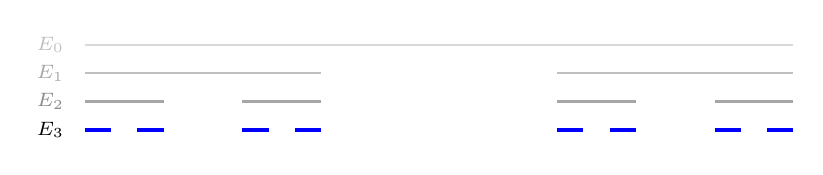
\begin{tikzpicture}[scale=9]
    % E_0 (lightest gray)
    \draw[thick, gray!30] (0,0.12) -- (1,0.12);
    \node[gray!50, left=4pt] at (0,0.12) {\scriptsize $E_0$};
    % E_1
    \draw[thick, gray!50] (0,0.08) -- (1/3,0.08);
    \draw[thick, gray!50] (2/3,0.08) -- (1,0.08);
    \node[gray!70, left=4pt] at (0,0.08) {\scriptsize $E_1$};
    % E_2
    \draw[thick, gray!70] (0,0.04) -- (1/9,0.04);
    \draw[thick, gray!70] (2/9,0.04) -- (3/9,0.04);
    \draw[thick, gray!70] (6/9,0.04) -- (7/9,0.04);
    \draw[thick, gray!70] (8/9,0.04) -- (1,0.04);
    \node[gray!90, left=4pt] at (0,0.04) {\scriptsize $E_2$};
    % E_3 (current stage, blue)
    \draw[very thick, blue] (0,0) -- (1/27,0);
    \draw[very thick, blue] (2/27,0) -- (3/27,0);
    \draw[very thick, blue] (6/27,0) -- (7/27,0);
    \draw[very thick, blue] (8/27,0) -- (9/27,0);
    \draw[very thick, blue] (18/27,0) -- (19/27,0);
    \draw[very thick, blue] (20/27,0) -- (21/27,0);
    \draw[very thick, blue] (24/27,0) -- (25/27,0);
    \draw[very thick, blue] (26/27,0) -- (1,0);
    \node[left=4pt] at (0,0) {\scriptsize $E_3$};
  \end{tikzpicture}
  \end{center}

  \note{
    Continuing this process forever, we get an infinite decreasing
    sequence of compact sets "E" sub "n". Two properties are worth
    recording. Property "a": the sets are nested. Property "b": at stage
    "n" we have 2 to the "n" disjoint closed intervals, each of length 1
    over 3 to the "n". The picture shows the first four stages stacked;
    notice how quickly the set shatters into many tiny pieces, even
    though the total length is shrinking geometrically to zero.
  }
\end{frame}

% =============================================================================
% --- The Cantor Set Definition ---
% =============================================================================

\begin{frame}{The Cantor Set}
  \begin{defblock}{Definition}
    The \alert{Cantor set} is
    \[
      P = \bigcap_{n=1}^{\infty} E_n.
    \]
  \end{defblock}

  \vspace{0.8em}
  \textbf{Basic properties:}
  \begin{itemize}
    \item Each $E_n$ is closed and bounded, so \alert{compact}.
    \item $P$ is an intersection of compact sets $\Longrightarrow$ $P$ is \alert{compact}.
    \item By the Corollary to Theorem 2.36: $P \neq \emptyset$.
  \end{itemize}

  \note{
    The Cantor set "P" is the intersection of all the stages "E" sub "n"
    as "n" ranges over the positive integers. In other words, "P" is the
    set of points that are never removed, no matter how many middle
    thirds we delete. Since each "E" sub "n" is a finite union of closed
    intervals, it is closed and bounded, hence compact. An intersection
    of compact sets is compact, so "P" is compact. Moreover, the "E" sub
    "n" form a nested decreasing sequence of nonempty compact sets, so by
    the corollary to Theorem 2.36 their intersection "P" is nonempty.
    The endpoints of the intervals at every stage, such as 0 and 1,
    clearly lie in "P", so we even have concrete members.
  }
\end{frame}

% =============================================================================
% --- P contains no segment (build 1/2) ---
% =============================================================================

% --- Build 1/2 ---
\begin{frame}{$P$ Contains No Segment}
  \textbf{Claim:} The Cantor set $P$ contains no segment $(\alpha,\beta)$.

  \vspace{0.8em}
  \textbf{Removed segments:} At stage $m$, we removed all segments of the form
  \[
    \left(\frac{3k+1}{3^m},\,\frac{3k+2}{3^m}\right), \tag{24}
  \]
  where $k,m$ are positive integers. These segments are \alert{disjoint from $P$}.

  \note{
    The Cantor set has a striking smallness property: it contains no open
    interval at all. The key observation is that the segments we remove at
    stage "m" have a very specific arithmetic form, shown on the slide as
    equation 24. They are the middle-third gaps, and there is one for each
    value of "k" and "m" with "k" running over appropriate integers. Every
    such segment was deleted in the construction, so none of them meets
    "P".
  }
\end{frame}

% --- Build 2/2 ---
\begin{frame}{$P$ Contains No Segment}
  \textbf{Claim:} The Cantor set $P$ contains no segment $(\alpha,\beta)$.

  \vspace{0.8em}
  \textbf{Removed segments:} At stage $m$, we removed all segments of the form
  \[
    \left(\frac{3k+1}{3^m},\,\frac{3k+2}{3^m}\right). \tag{24}
  \]

  \vspace{0.4em}
  \textbf{Every segment $(\alpha,\beta)$ contains one of form (24)}: pick $m$ so that
  \[
    3^{-m} < \frac{\beta-\alpha}{6}.
  \]
  Hence $(\alpha,\beta) \not\subset P$. \hfill \alert{$\boxed{P \text{ contains no segment.}}$}

  \note{
    Now take any open segment with endpoints alpha and beta, no matter how
    short, and choose "m" so large that 1 over 3 to the "m" is smaller
    than one sixth of the length of that segment. At stage "m" the grid
    spacing is small enough that some removed middle-third interval,
    shown on the slide as equation 24, fits entirely inside alpha beta.
    Since that removed interval is disjoint from "P", our segment alpha
    beta cannot be a subset of "P" either. So the Cantor set contains no
    open interval at all. Topologically it is extremely thin.
  }
\end{frame}

% =============================================================================
% --- P is perfect: strategy ---
% =============================================================================

\begin{frame}{$P$ is Perfect: Strategy}
  \textbf{$P$ is closed} --- intersection of closed sets. \\
  So we only need to show $P$ has \alert{no isolated point}.

  \vspace{0.6em}
  \textbf{Plan:} For every $x \in P$ and every segment $S$ containing $x$, find another point of $P$ in $S$.

  \vspace{0.6em}
  \textbf{Key trick:} The endpoints of each stage's intervals are \emph{never removed}, so they all lie in $P$.

  \note{
    To show that "P" is perfect, we first note that "P" is closed, since
    it is an intersection of closed sets. So perfection comes down to
    showing that no point of "P" is isolated. Concretely, we must show
    that given any point "x" of "P" and any open segment "S" containing
    "x", there is another point of "P" in "S" different from "x". The
    secret is this: the endpoints of the intervals at each stage of the
    construction are never removed, because we only remove open middle
    thirds, and endpoints stay. So endpoints are a rich supply of points
    already guaranteed to be in "P". We will use a very close endpoint as
    our witness.
  }
\end{frame}

% =============================================================================
% --- P is perfect: details ---
% =============================================================================

\begin{frame}{$P$ is Perfect: The Argument}
  Let $x \in P$ and let $S$ be any segment containing $x$.

  \vspace{0.5em}
  Let $I_n$ be the interval of $E_n$ that contains $x$.
  \begin{itemize}
    \item $I_n$ has length $3^{-n} \to 0$.
    \item Choose $n$ large enough so $I_n \subset S$.
  \end{itemize}

  \vspace{0.3em}
  Let $x_n$ be an endpoint of $I_n$ with $x_n \neq x$.
  \begin{itemize}
    \item $x_n \in P$ (endpoints are never removed).
    \item $x_n \in I_n \subset S$.
  \end{itemize}

  \vspace{0.2em}
  \alert{$\Longrightarrow$ $x$ is a limit point of $P$.}

  \note{
    Fix "x" in "P" and any segment "S" around "x". For each stage "n", let
    "I" sub "n" be the one interval of "E" sub "n" that contains "x"; at
    every stage there is exactly one such interval, because "x" lies in
    "P" and therefore in "E" sub "n". The length of "I" sub "n" is 1 over
    3 to the "n", which goes to zero, so for "n" large enough "I" sub "n"
    sits entirely inside "S". Now pick any endpoint of "I" sub "n" other
    than "x", and call it "x" sub "n". That endpoint is in "P" because
    endpoints of the construction are never removed, and it is in "I" sub
    "n", hence in "S". So we have found a point of "P" different from "x"
    inside every segment around "x". Therefore "x" is a limit point of
    "P". Since "x" was arbitrary, "P" has no isolated points, and "P" is
    perfect.
  }
\end{frame}

% =============================================================================
% --- Perfect diagram ---
% =============================================================================

\begin{frame}{Visualizing Why $P$ is Perfect}
  \begin{center}
  \begin{tikzpicture}[scale=1.0]
    % A schematic zoom into stage n near x
    % E_n: three visible blue intervals, with I_n in the middle
    \draw[very thick, blue] (-5.5,0) -- (-4.5,0);
    \draw[very thick, blue] (-1.2,0) -- (1.2,0);   % I_n (wide so labels fit)
    \draw[very thick, blue] (4.5,0) -- (5.5,0);
    \node[blue, left=4pt] at (-5.5,0) {\scriptsize stage $E_n$};

    % Segment S (wider than I_n, centered on x) -- open segment, hollow endpoints
    \draw[thick, mAccent] (-4.4,-1.7) -- (2.0,-1.7);
    \draw[thick, mAccent, fill=white] (-4.4,-1.7) circle (3pt);
    \draw[thick, mAccent, fill=white] (2.0,-1.7) circle (3pt);
    \node[mAccent, below=4pt] at (-1.2,-1.7) {$S$};

    % Vertical dashed red line connecting x to the center of S
    \draw[dashed, red] (-1.2,0) -- (-1.2,-1.7);

    % Brace for I_n under the middle blue interval
    \draw[thick, mDarkTeal, decorate, decoration={brace,amplitude=5pt,mirror}]
      (-1.2,-0.15) -- (1.2,-0.15);
    \node[mDarkTeal, below=8pt] at (0,-0.15) {\scriptsize $I_n$ (length $3^{-n}$)};

    % x and x_n as the endpoints of I_n
    \fill[red] (-1.2,0) circle (3pt);
    \node[red, above=3pt] at (-1.2,0) {$x$};

    \fill[mAccent] (1.2,0) circle (3pt);
    \node[mAccent, above=3pt] at (1.2,0) {$x_n$};
  \end{tikzpicture}
  \end{center}

  \vspace{0.2em}
  \centerline{\scriptsize Choose $n$ large enough that $I_n \subset S$.}

  \note{
    Here is a schematic picture of the argument. The three blue bars at
    the top represent a few surviving intervals of "E" sub "n" near our
    point. Because "x" lies in "P", it sits inside exactly one of these
    intervals at every stage; that interval is labeled "I" sub "n" and is
    the middle blue bar, marked with a brace below for emphasis. Its
    length is 1 over 3 to the "n", which we can make as small as we like
    by taking "n" large. Below the blue intervals, the orange line with
    hollow endpoints is our given open segment "S", drawn centered on "x"
    for clarity; the dashed red line drops from "x" to the center of "S"
    to highlight that alignment. Once "n" is large enough, the short
    interval "I" sub "n" fits entirely inside "S". The red dot marks "x"
    at the left end of "I" sub "n", and the orange dot marks the other
    endpoint, which we call "x" sub "n". Because "x" sub "n" is a
    construction endpoint, it is never removed, so it lies in "P"; and
    since "I" sub "n" is inside "S", it also lies in "S". So inside any
    segment around "x" we can always find another point of "P", which
    is exactly what it means for "x" to be a limit point.
  }
\end{frame}

% =============================================================================
% --- Remark: Uncountable Measure Zero ---
% =============================================================================

\begin{frame}{The Cantor Set: A Striking Object}
  \begin{remblock}{Final observations on 2.44}
    Combining everything we now know:
  \end{remblock}

  \vspace{0.5em}
  \begin{itemize}
    \item $P$ is \alert{perfect} and nonempty $\Longrightarrow$ by Theorem 2.43, $P$ is \alert{uncountable}.
    \item $P$ contains \alert{no segment} --- topologically ``tiny''.
    \item Total length removed:
      $\displaystyle \frac{1}{3} + \frac{2}{9} + \frac{4}{27} + \cdots = \sum_{n=0}^{\infty}\frac{2^n}{3^{n+1}} = 1$.
    \item $P$ has \alert{measure zero} --- yet is uncountable (see Chap.~11).
  \end{itemize}

  \note{
    Let us take stock. The Cantor set "P" is perfect and nonempty, so by
    our main theorem it is uncountable, so it has as many points as the
    real line. On the other hand, "P" contains no open segment, so it is
    topologically extremely thin. We can even compute the total length
    removed during the construction: at stage 1 we remove one piece of
    length 1 third, at stage 2 we remove two pieces each of length 1
    ninth, and so on. The total is a geometric series that sums to 1, so
    nothing is left in the sense of length. In Chapter 11 we will see
    that this means the Cantor set has Lebesgue measure zero. So "P" is
    an uncountable set of measure zero, simultaneously as big as the
    reals and as small as a single point from the measure-theoretic
    perspective. This is one of the reasons the Cantor set is so
    important.
  }
\end{frame}

% =============================================================================
% --- Summary ---
% =============================================================================

\begin{frame}{Summary}
  \textbf{Key takeaways from this section:}
  \begin{itemize}
    \item \alert{Theorem 2.43}: every nonempty perfect set in $\mathbb{R}^k$ is uncountable.
    \item Proof technique: nested shrinking neighborhoods + compactness (Cor.\ 2.36).
    \item \alert{Corollary}: every interval $[a,b]$ with $a<b$ is uncountable, so $\mathbb{R}$ is uncountable.
    \item \alert{Cantor set} $P = \bigcap_n E_n$ is:
      \begin{itemize}
        \item compact, nonempty, \emph{perfect},
        \item contains \emph{no segment},
        \item uncountable, measure zero.
      \end{itemize}
  \end{itemize}

  \vspace{0.4em}
  \textbf{Coming up:} Connected sets --- when is a set ``in one piece''?

  \note{
    To summarize, the main theorem of this section is that every nonempty
    perfect subset of Euclidean space is uncountable. The proof used a
    clever construction of nested shrinking neighborhoods, each one
    designed to kick out one listed point, together with the compactness
    corollary of Theorem 2.36. A direct corollary is that every
    nondegenerate closed interval and therefore the whole real line are
    uncountable. We then built the Cantor set by repeatedly removing
    middle thirds from the unit interval. The resulting set is compact,
    nonempty, contains no segment, yet is perfect and therefore
    uncountable. It also has Lebesgue measure zero, as we will see in
    Chapter 11. In the next section we turn to connectedness, the precise
    notion of a set being in one piece. See you there.
  }
\end{frame}

\end{document}
